\documentclass[]{article}
\usepackage[spanish.mexico]{babel}
\usepackage[T1]{fontenc}
\usepackage[utf8]{inputenc}
%\usepackage{lmodern}
\usepackage[a4paper]{geometry}

\usepackage{amsmath}


%Graficos e imagenes
\usepackage{graphicx}
%\graphicspath{ Imagenes/ }

\usepackage{cite}

%Grafico de barras
%\usepackage{pgfplots}


\usepackage{tikz}
\usepackage[american voltages, american currents,siunitx]{circuitikz}

%\title{Proyecto de Optimización de Energía}
%\author{Pablo Vivar Colina}
%\date{Mayo 2018}



\begin{document}
	
%\usepackage[top=2cm,bottom=2cm,left=1cm,right=1cm]{geometry}


\begin{titlepage}
     \begin{center}
	
\includegraphics[width=0.09\textwidth]{UNAM}\Large Universidad Nacional Autónoma de México
        	
\includegraphics[width=0.09\textwidth]{FI}\\[1cm]
        \Large Facultad de Ingeniería\\[1cm]
       % \Large División de Ciencias Básicas\\[1cm]
         \Large Laboratorio de Fundamentos de Control(6655)\\[1cm]
         %la clave antes era:4314
         \footnotesize Profesor: Salcedo Ubilla María Leonor Ing.\\[1cm]
        \footnotesize Semestre 2019-1\\[1cm]
        
       

        \Large Práctica No. 1\\[1cm]
        
           

\Large Introdcción MATLAB
        
         %Texto a la derecha
          \begin{flushright}
\footnotesize  Grupo 2\\[0.5cm]
\footnotesize Brigada: 4\\[0.5cm]
\footnotesize Rodrigo Adrián Martínez López\\[0.5cm]
\footnotesize Vivar Colina Pablo\\[0.5cm]
 \end{flushright}
    %Texto a la izquierda
          \begin{flushleft}
        \footnotesize Ciudad Universitaria Agosto de 2018.\\
          \end{flushleft}
         
          
        %\vfill
        %\today
   \end{center}
\end{titlepage}
 %agregar portada

%\maketitle

\tableofcontents  % Write out the Table of Contents

%\listoffigures  % Write out the List of Figures

\section{Resumen}

\section{Introducción}

Sintonizar los parámetros de un controlador PID consiste en determinar el valor de la
constante de tiempo que les corresponde a cada uno de los controladores, es decir, se
debe determinar el valor de $kp$, el de $Ti$, y el de $Td$ para lograr que el sistema de control tenga un comportamiento aceptable y robusto, en conformidad con los criterios de
desempeño establecidos para el sistema.\\

Existen diversos métodos para ello, mas en los sistemas de ajuste de malla cerrada no
es necesario conocer los parámetros de la función de transferencia que caracterizan al
sistema.\\

El Método Harriot, se usa cuando el proceso no se puede llevar a una oscilación
sostenida.\\

Este método consiste en crear un sistema en malla cerrada con un controlador
proporcional puro donde los otros dos no tienen influencia alguna, después se va
incrementando el valor de la ganancia del P hasta que se obtiene una curva donde la
proporción del primer sobre paso y el segundo es del 25 porciento.\\

 De esa curva solo se
anota el valor del periodo P con el que se dan ambas oscilaciones. Con el periodo P se
calculan las constantes de tiempo Ti y Td, usando las siguientes formulas; $Ti = \frac{P}{6}$,
$Td=\frac{P}{1.5}$, de acuerdo con la siguiente tabla. Después se hace funcionar el sistema con
los valores calculados de TI y Td, y nuevamente se ajusta la ganancia a la misma razón
de $\frac{1}{4}$ en la respuesta. La ganancia así obtenida será el valor usado para el $Kp$ en el
controlador.\\


\subsection{NI ELVIS}

Para crear una aplicación completa de NI ELVIS, explore otras soluciones de laboratorio para NI ELVIS.\\

Proporciona una experiencia de aprendizaje basada en proyectos, usando medidas en línea y diseño práctico y embebido.\\

El NI Educational Laboratory Virtual Instrumentation Suite (NI ELVIS) es un dispositivo modular de laboratorio educativo de ingeniería desarrollado específicamente para la academia. Con este enfoque práctico, los profesores pueden ayudar a los estudiantes a aprender habilidades de ingeniería prácticas y experimentales. NI ELVIS incluye un osciloscopio, multímetro digital, generador de funciones, fuente de alimentación variable, analizador de Bode y otros instrumentos comunes de laboratorio. Puede conectar una PC al NI ELVIS usando USB y desarrollar circuitos en su protoboard desmontable.\cite{NationalInstruments2018}\\


\section{Objetivos}




\subsection{Generales}

\begin{itemize}
	\item El estudiante conocerá la estructura de los módulos G35 y TY35/EV.
\end{itemize}

\subsection{Específicos}

	\begin{itemize}
			\item Caracterizará el Transductor del Sistema.
			\item Comprenderá la operación analógica y digital del sistema de control
			de presión.
			\item Aplicará los conceptos de controlador Proporcional, Proporcional
			Integral Derivativo (PID), a un sistema analógico y a un sistema
			digital.
	\end{itemize}


\section{Materiales y métodos}

	\begin{itemize}
		\item NI Elvis
		\item Computadora con Suite de herramientas Texas Instruments
	\end{itemize}
	
\section{Resultados}



\begin{table}[h!]
	\centering
	\begin{tabular}{|c|c|c|}
		\hline
		Presión {[}bar{]} & Ventrada {[}V{]} & Vsalida {[}V{]} \\ \hline
		0                 & 0                & 0               \\ \hline
		0.2               & 0.764            & 0.888           \\ \hline
		0.4               & 1.373            & 1.513           \\ \hline
		0.6               & 1.787            & 1.935           \\ \hline
		0.8               & 2.245            & 2.399           \\ \hline
		1                 & 3.577            & 3.75            \\ \hline
		1.2               & 4.23             & 4.409           \\ \hline
		1.4               & 4.833            & 5.018           \\ \hline
		1.6               & 5.966            & 5.1966          \\ \hline
		1.8               & 7.14             & 7.35            \\ \hline
		2                 & 7.35             & 7.57            \\ \hline
	\end{tabular}
	\caption{Tabla}
\end{table}


\begin{table}[h!]
	\centering
	\begin{tabular}{|c|c|c|}
		\hline
		kc   & Ti    & Td   \\ \hline
		1.67 & 0.355 & 0.83 \\ \hline
		1.67 & 1     & 0.5  \\ \hline
		1.67 & 3     & 1    \\ \hline
		1.67 & 4     & 1.5  \\ \hline
		1.67 & 5     & 2    \\ \hline
	\end{tabular}
	\caption{Tabla}
\end{table}



%AQUI VAMOS




\begin{figure}[h!]
	\centering
	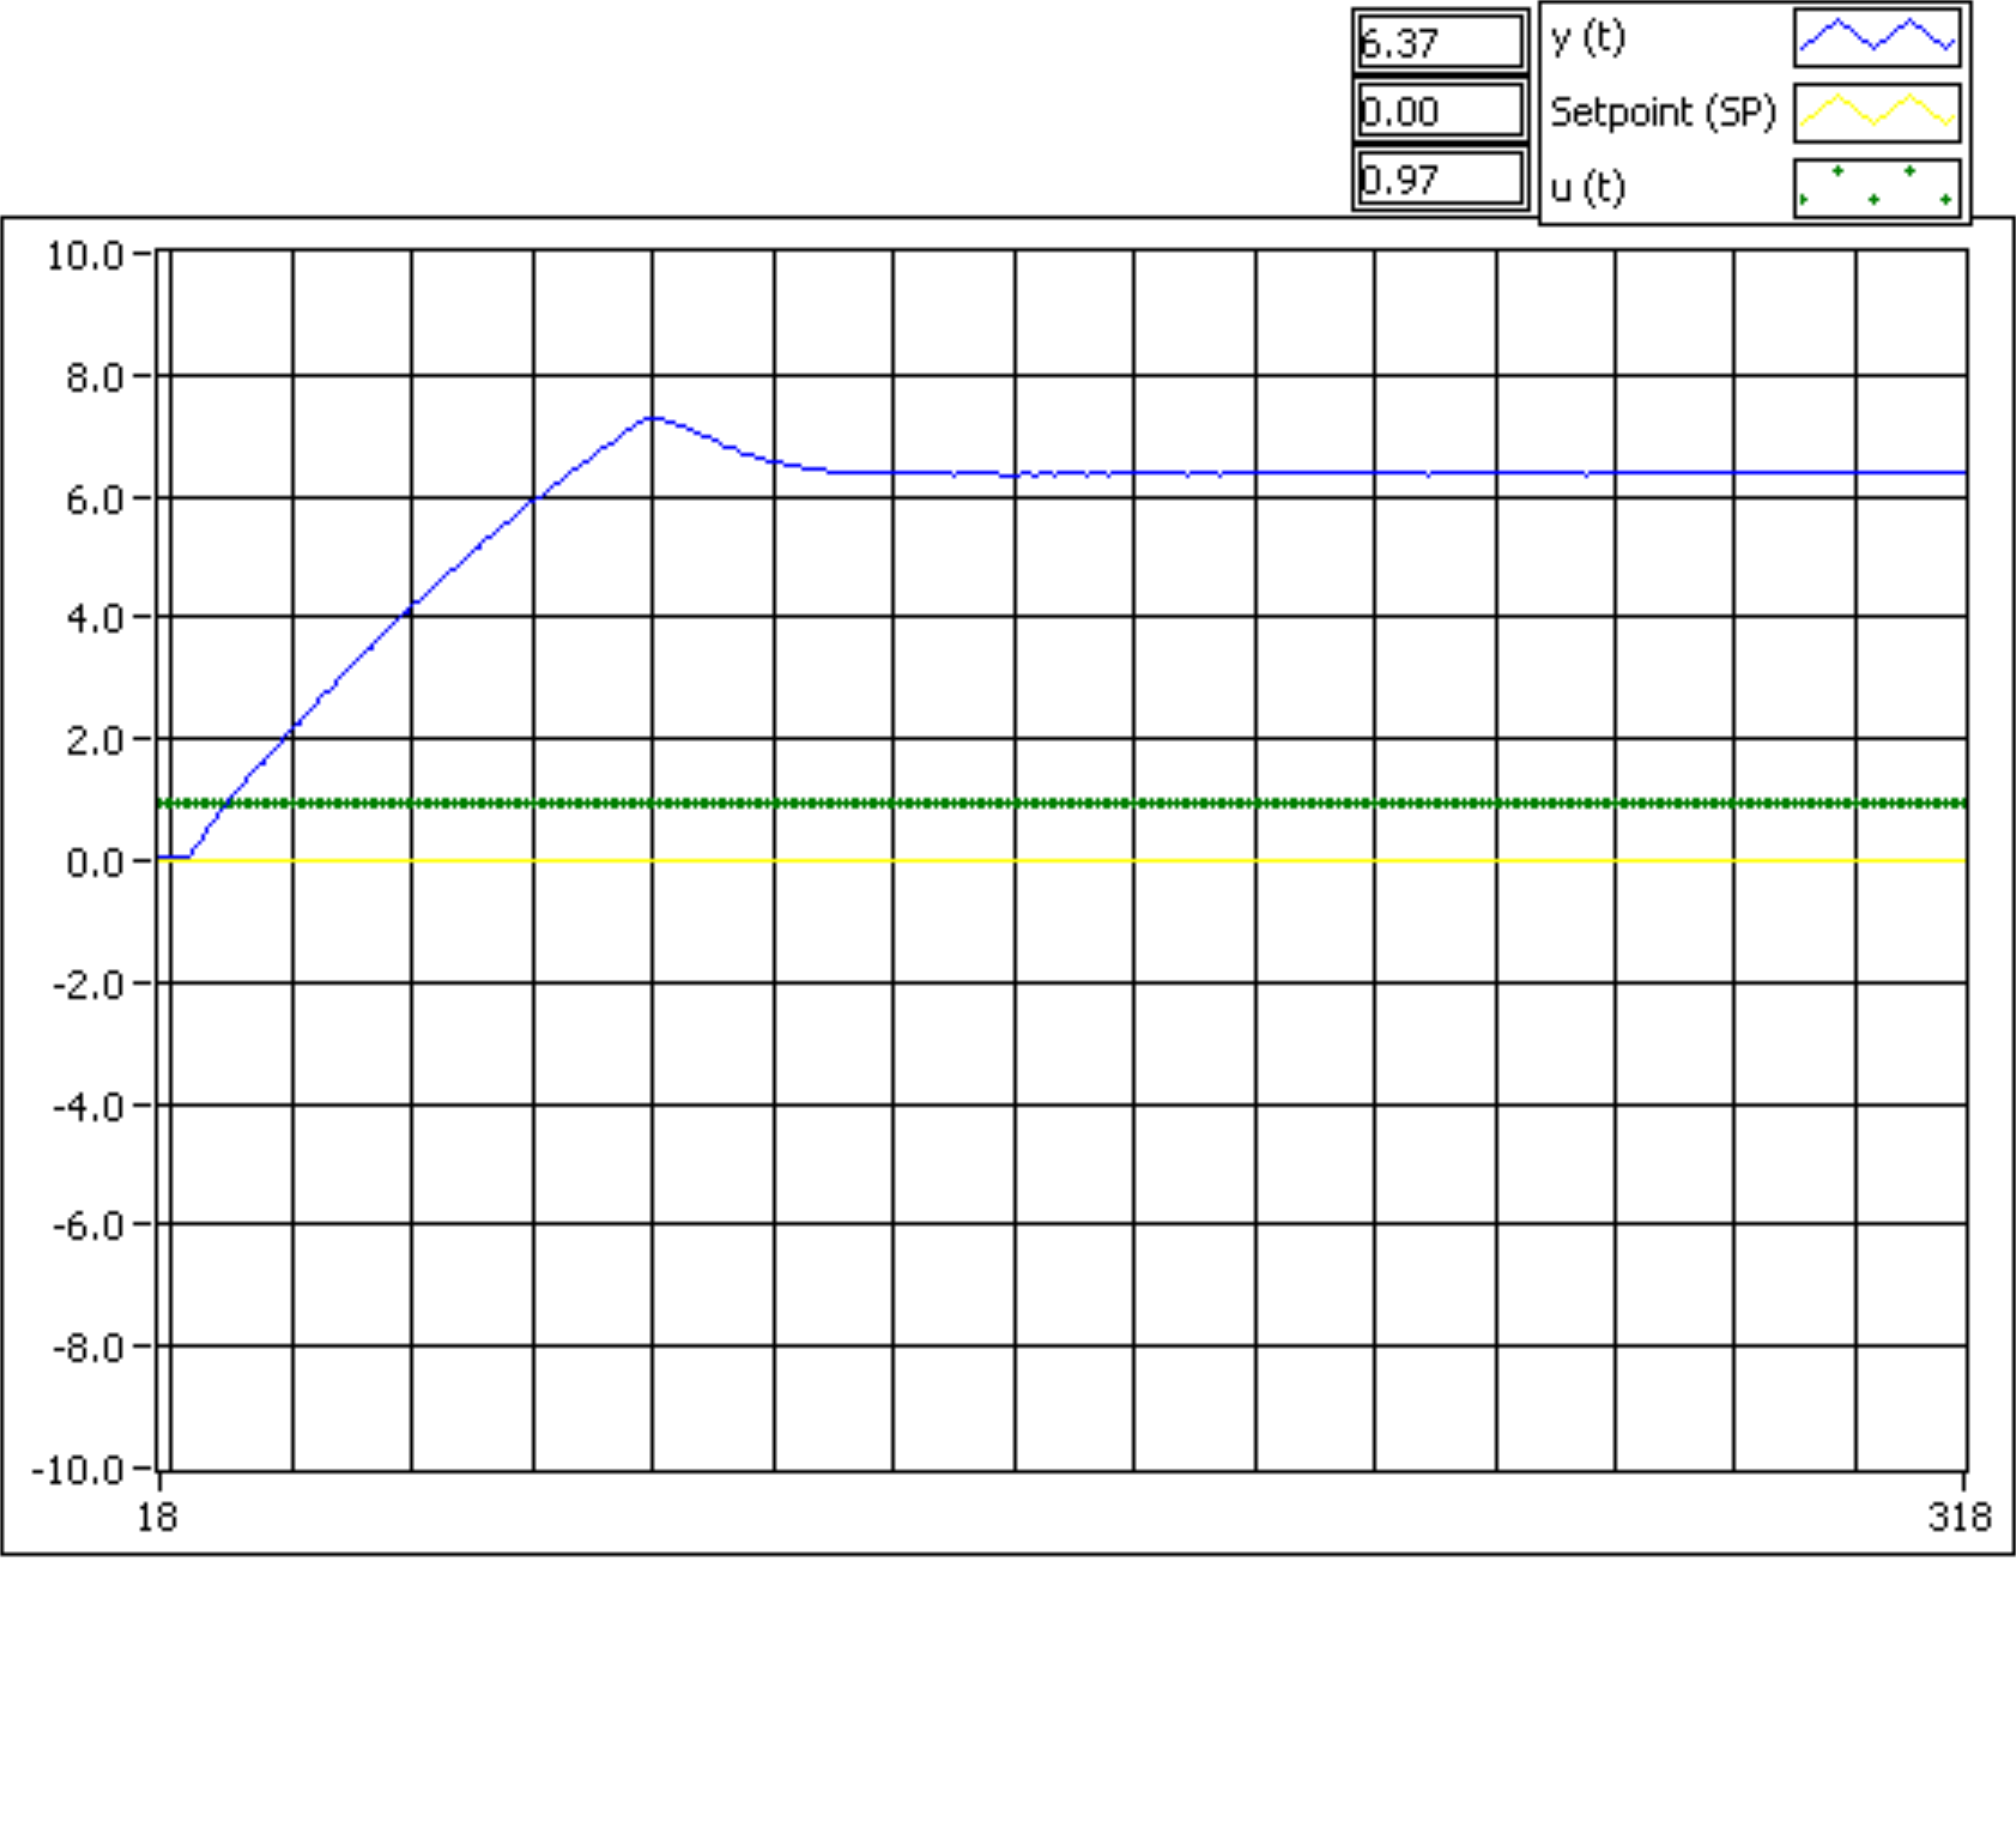
\includegraphics[width=0.6\textwidth]{Imagenes/ControlP_0.png}
	\caption{Control P 0}
	\label{fig:ControlP0}
\end{figure}

\begin{figure}[h!]
	\centering
	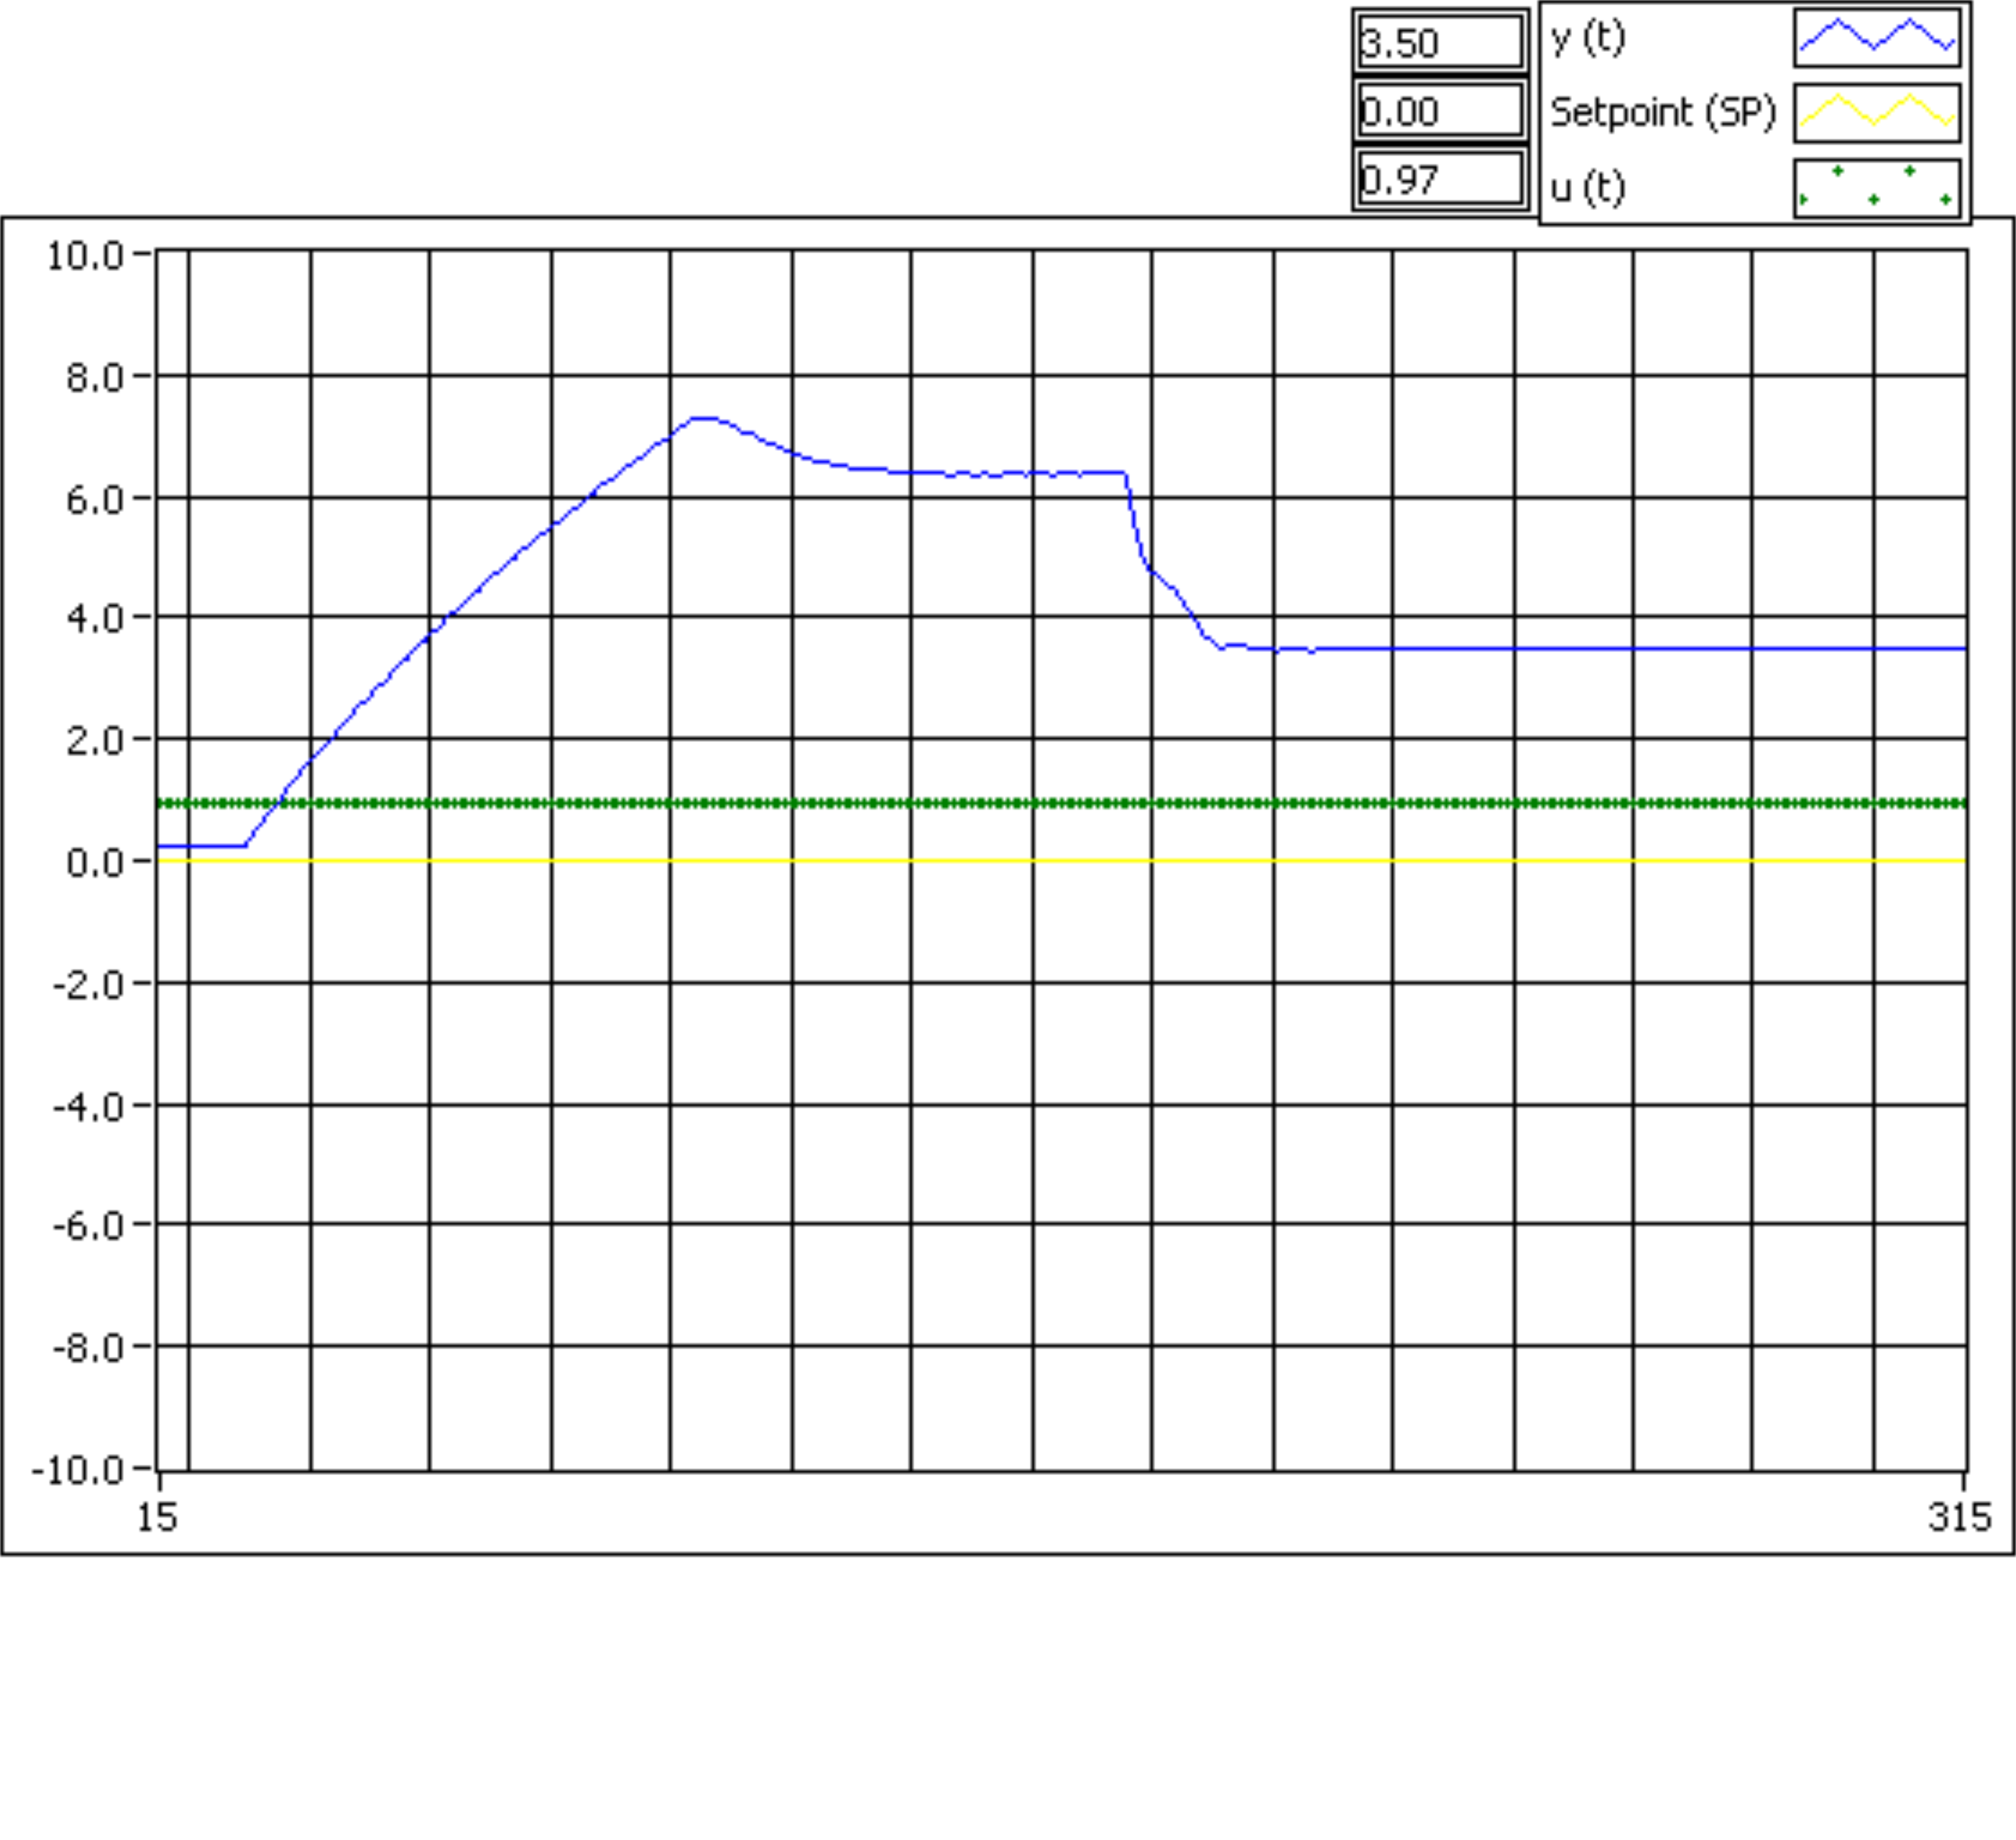
\includegraphics[width=0.6\textwidth]{Imagenes/ControlP.png}
	\caption{Control P}
	\label{fig:ControlP}
\end{figure}


\begin{figure}[h!]
	\centering
	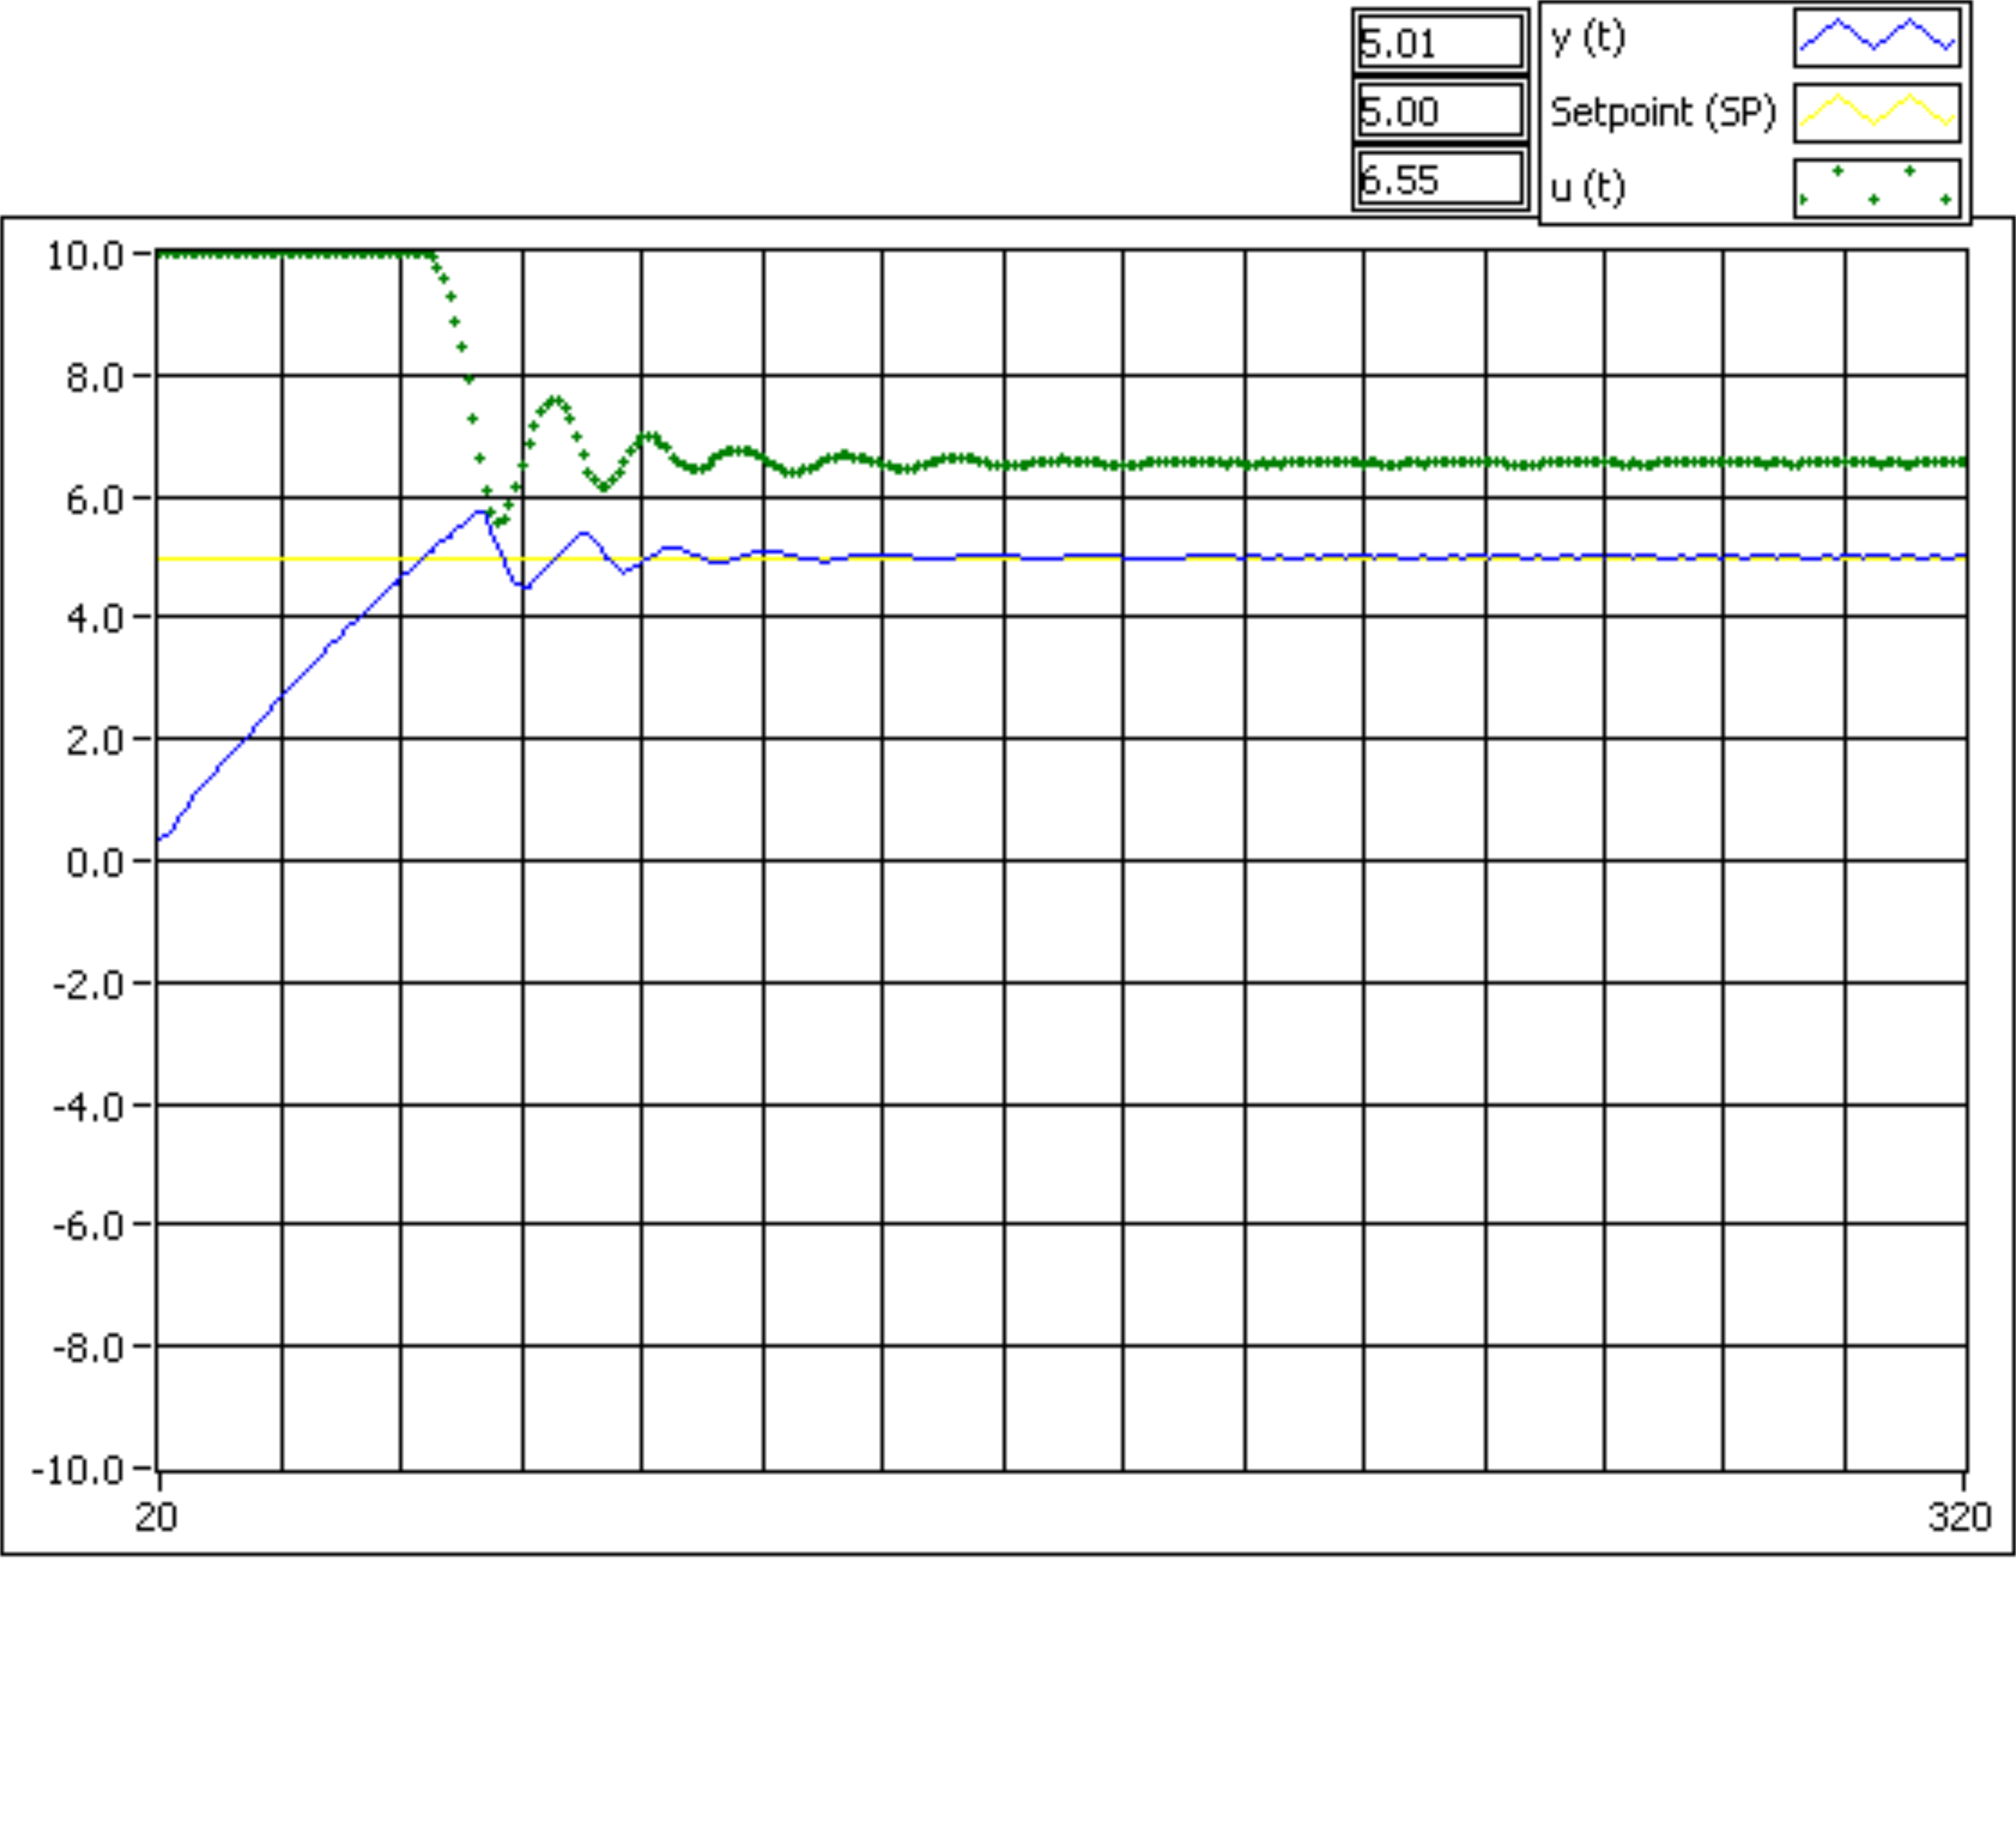
\includegraphics[width=0.6\textwidth]{Imagenes/DigitalA.png}
	\caption{Digital}
	\label{fig:DigitalA}
\end{figure}

\begin{figure}[h!]
	\centering
	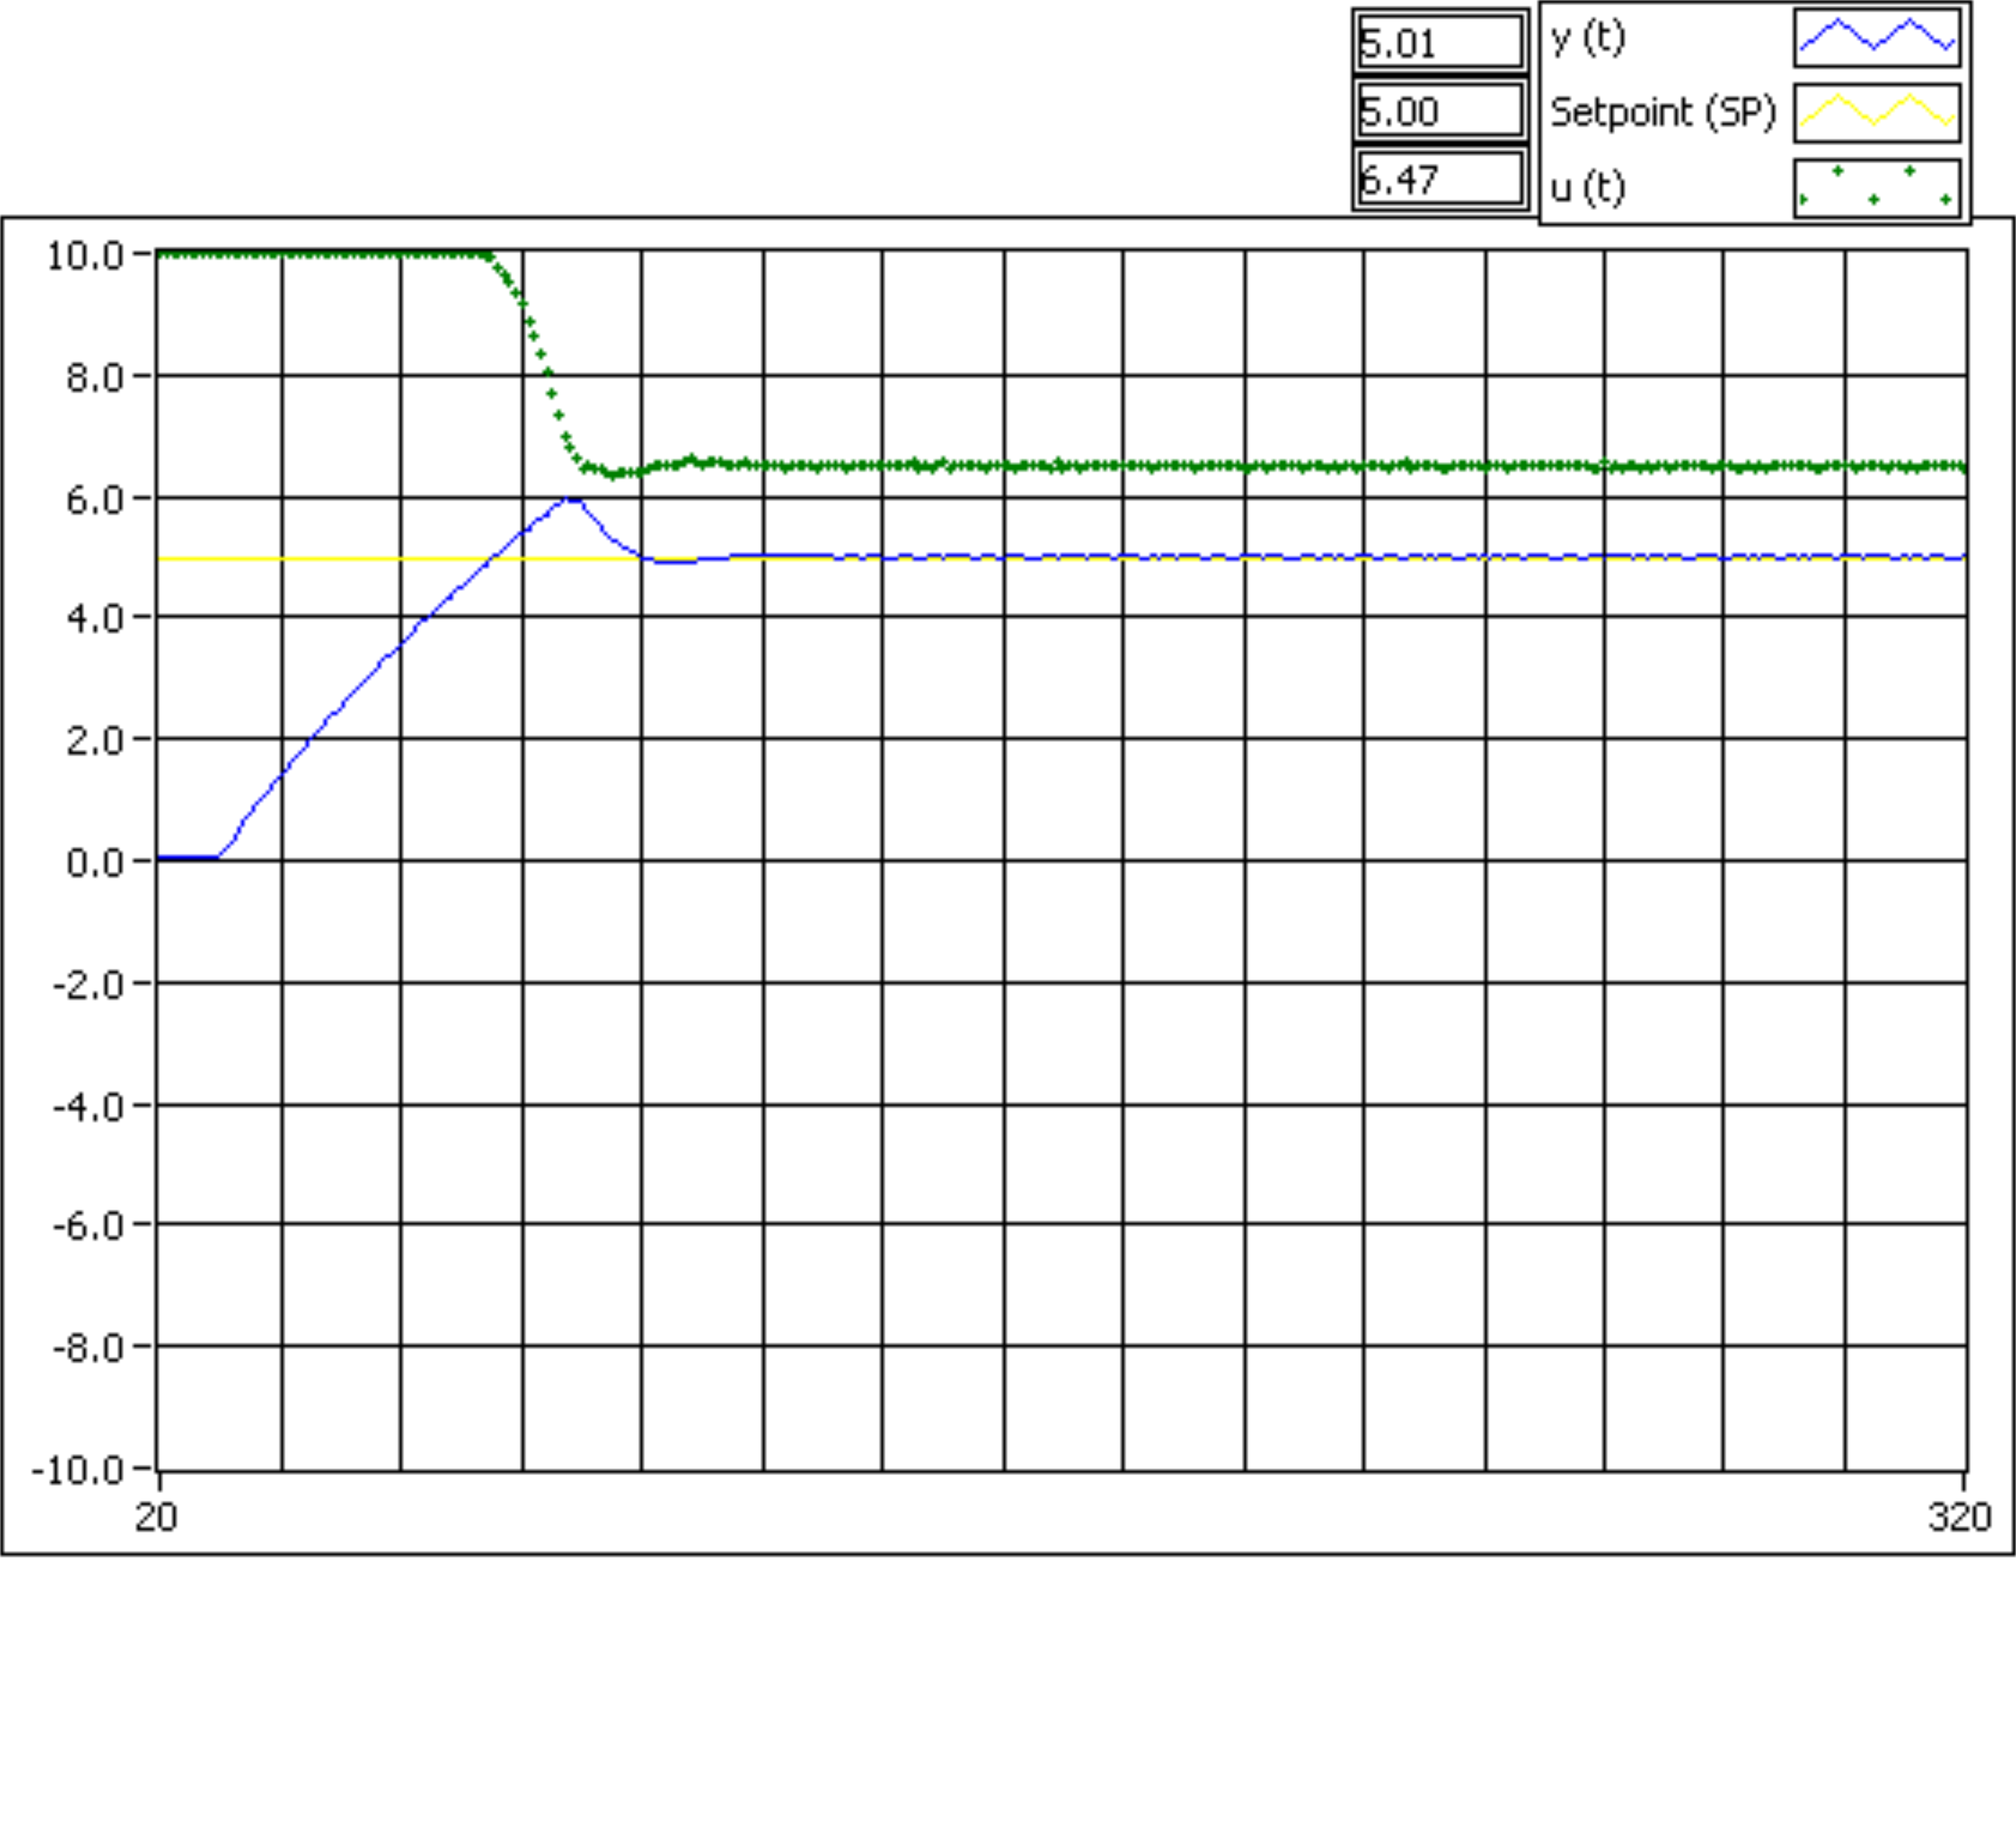
\includegraphics[width=0.6\textwidth]{Imagenes/DigitalB.png}
	\caption{Digital}
	\label{fig:DigitalB}
\end{figure}


\begin{figure}[h!]
	\centering
	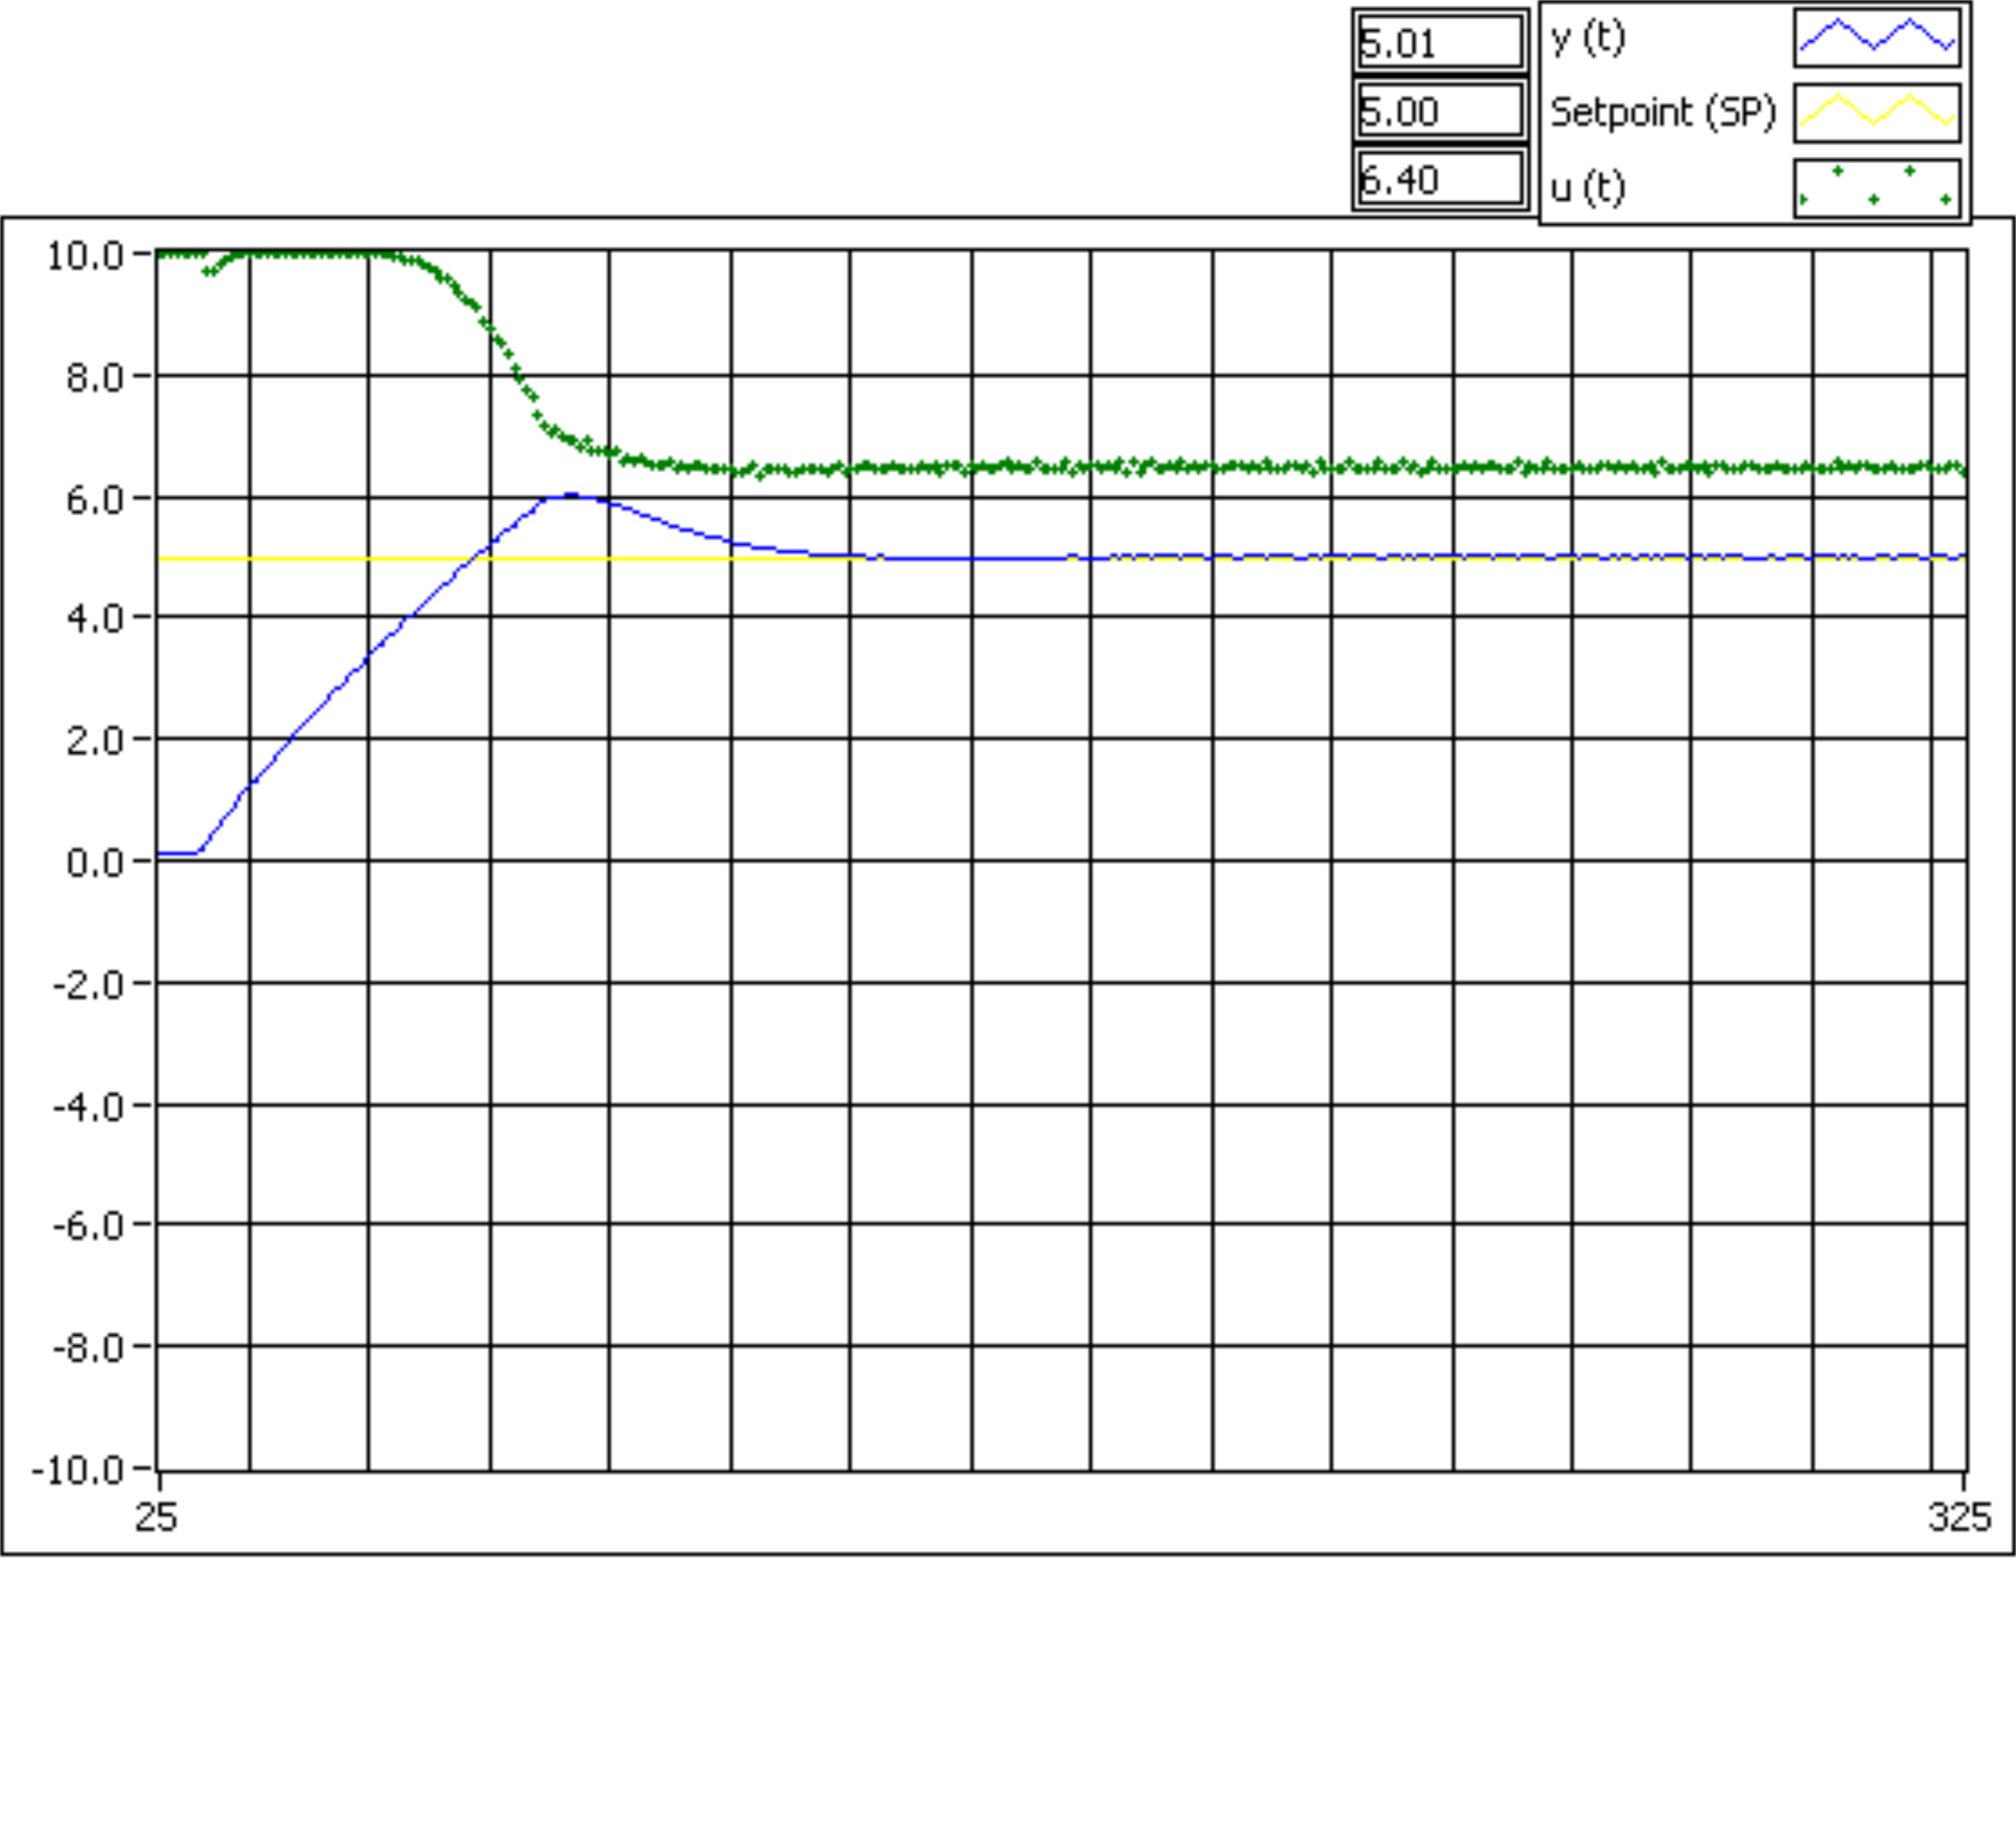
\includegraphics[width=0.6\textwidth]{Imagenes/DigitalC.png}
	\caption{Digital}
	\label{fig:DigitalC}
\end{figure}


\begin{figure}[h!]
	\centering
	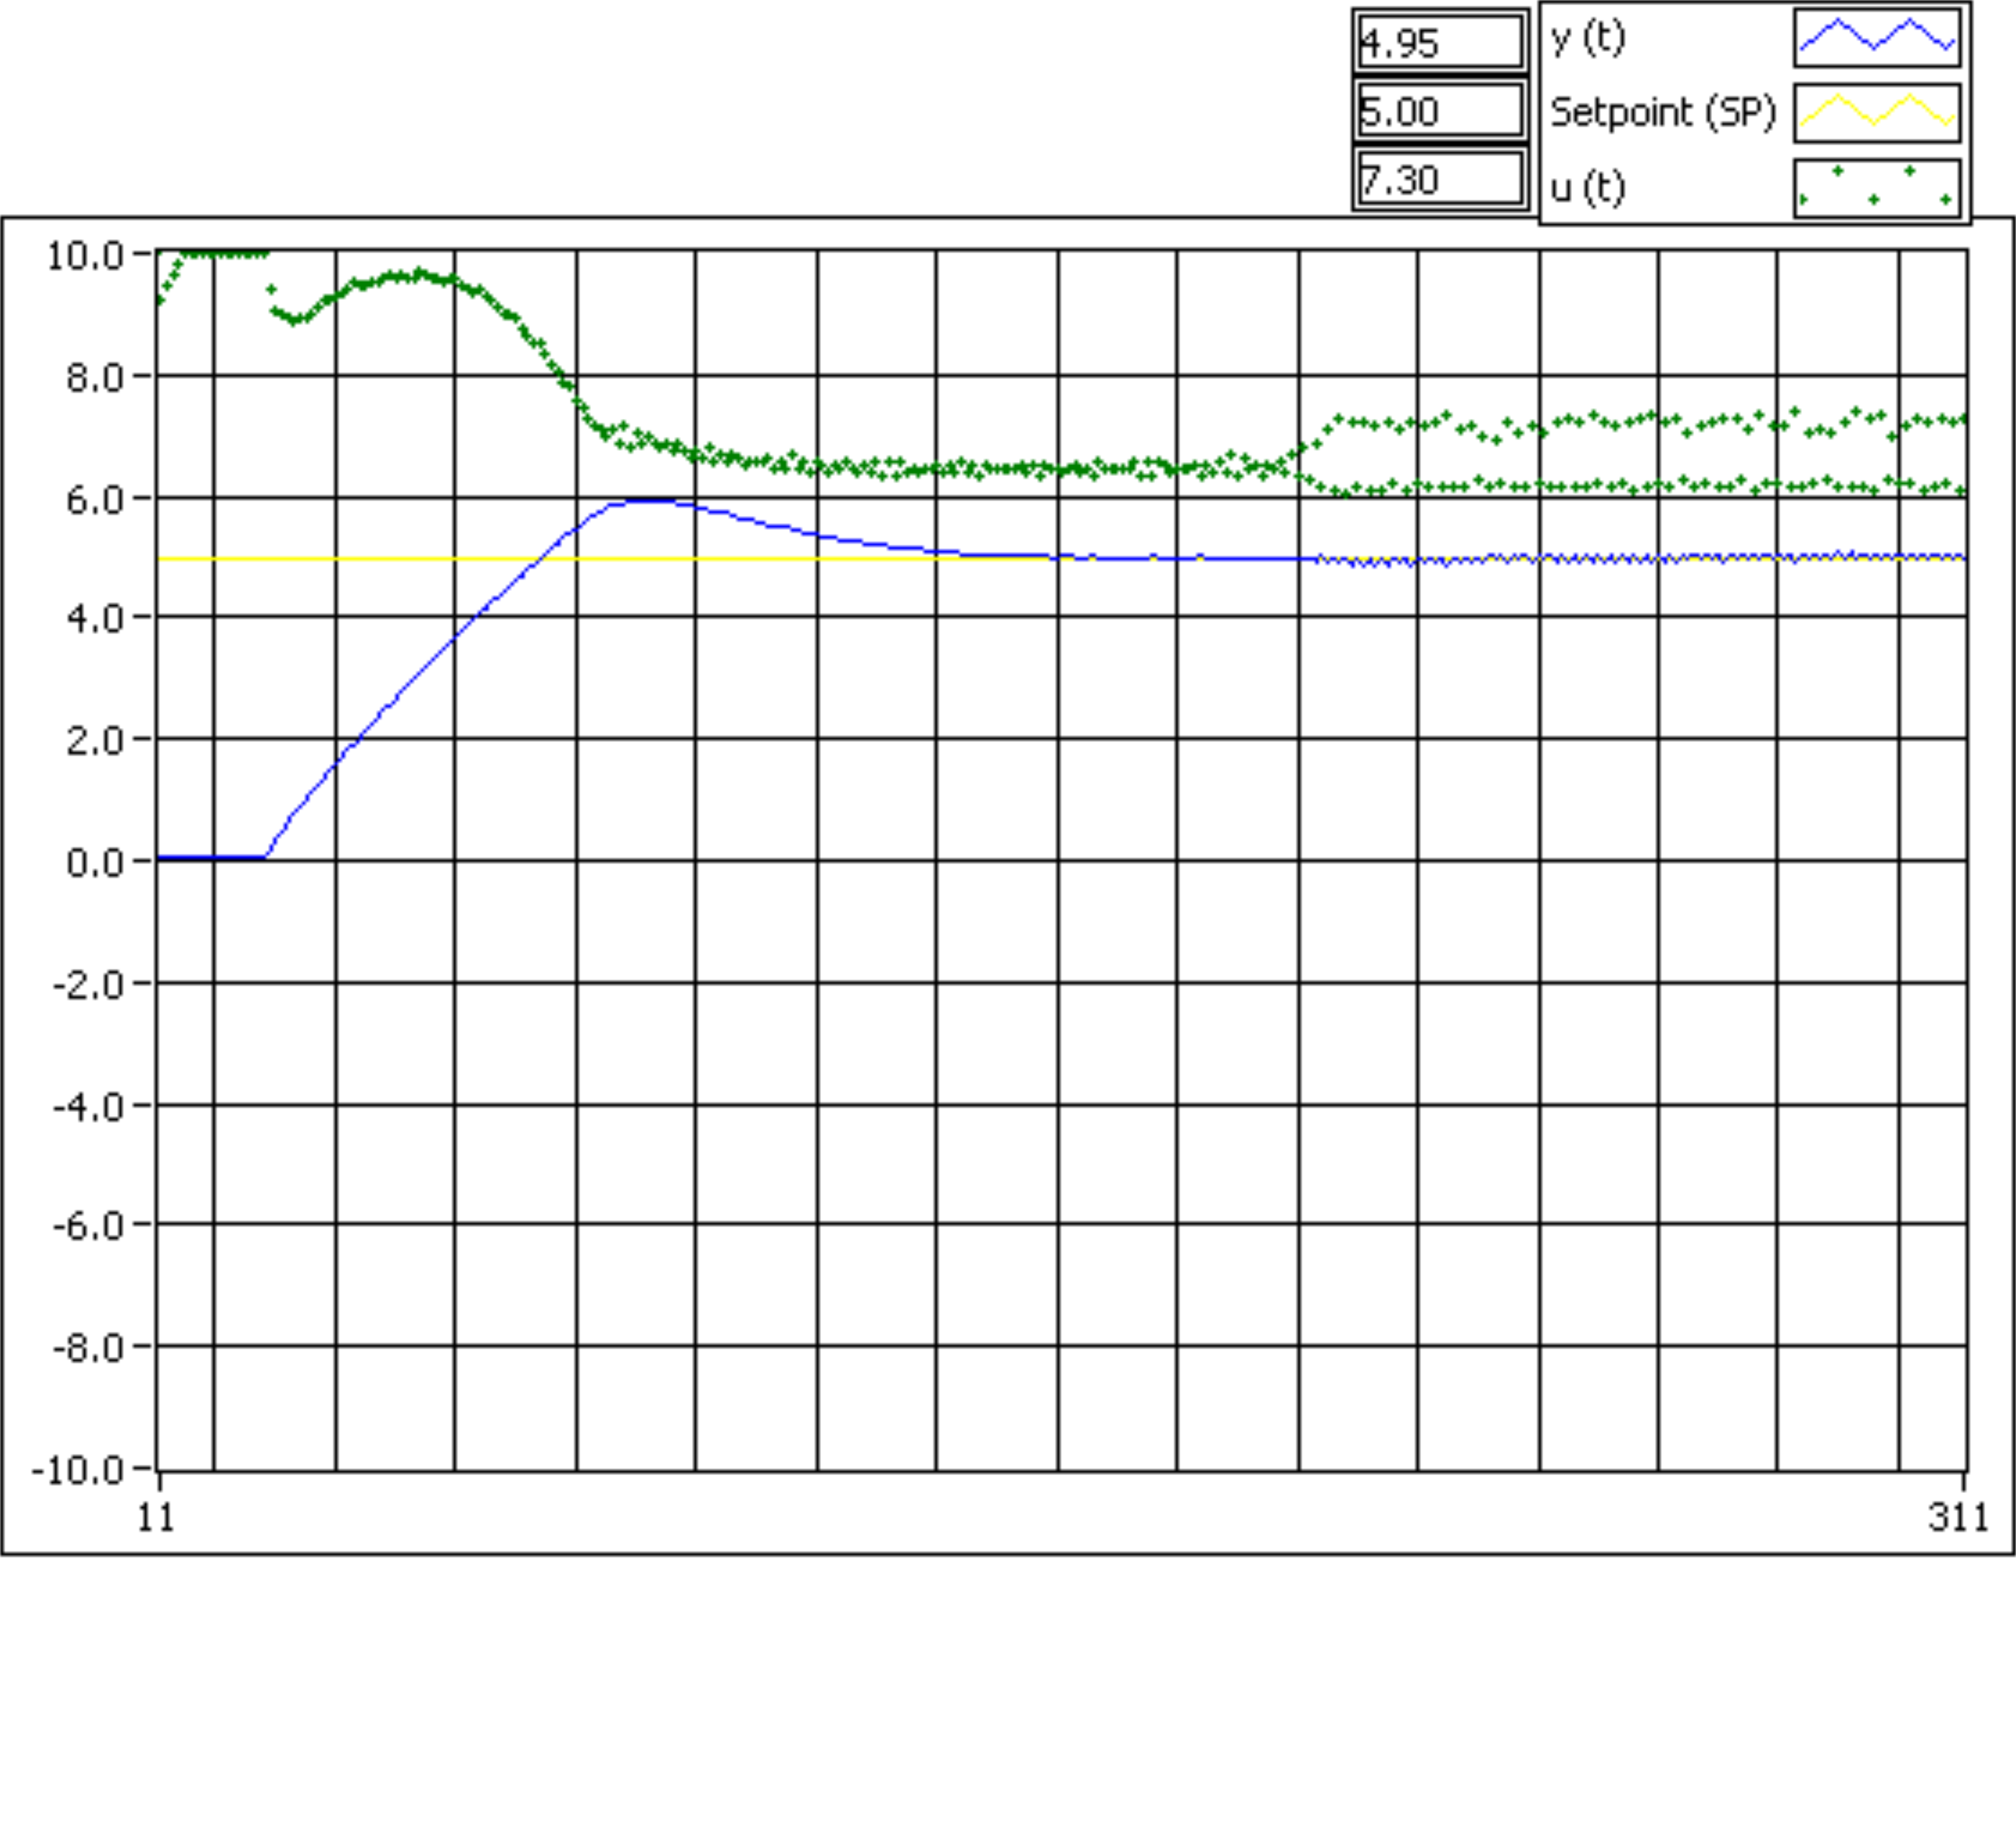
\includegraphics[width=0.6\textwidth]{Imagenes/DigitalD.png}
	\caption{Digital}
	\label{fig:DigitalD}
\end{figure}


\begin{figure}[h!]
	\centering
	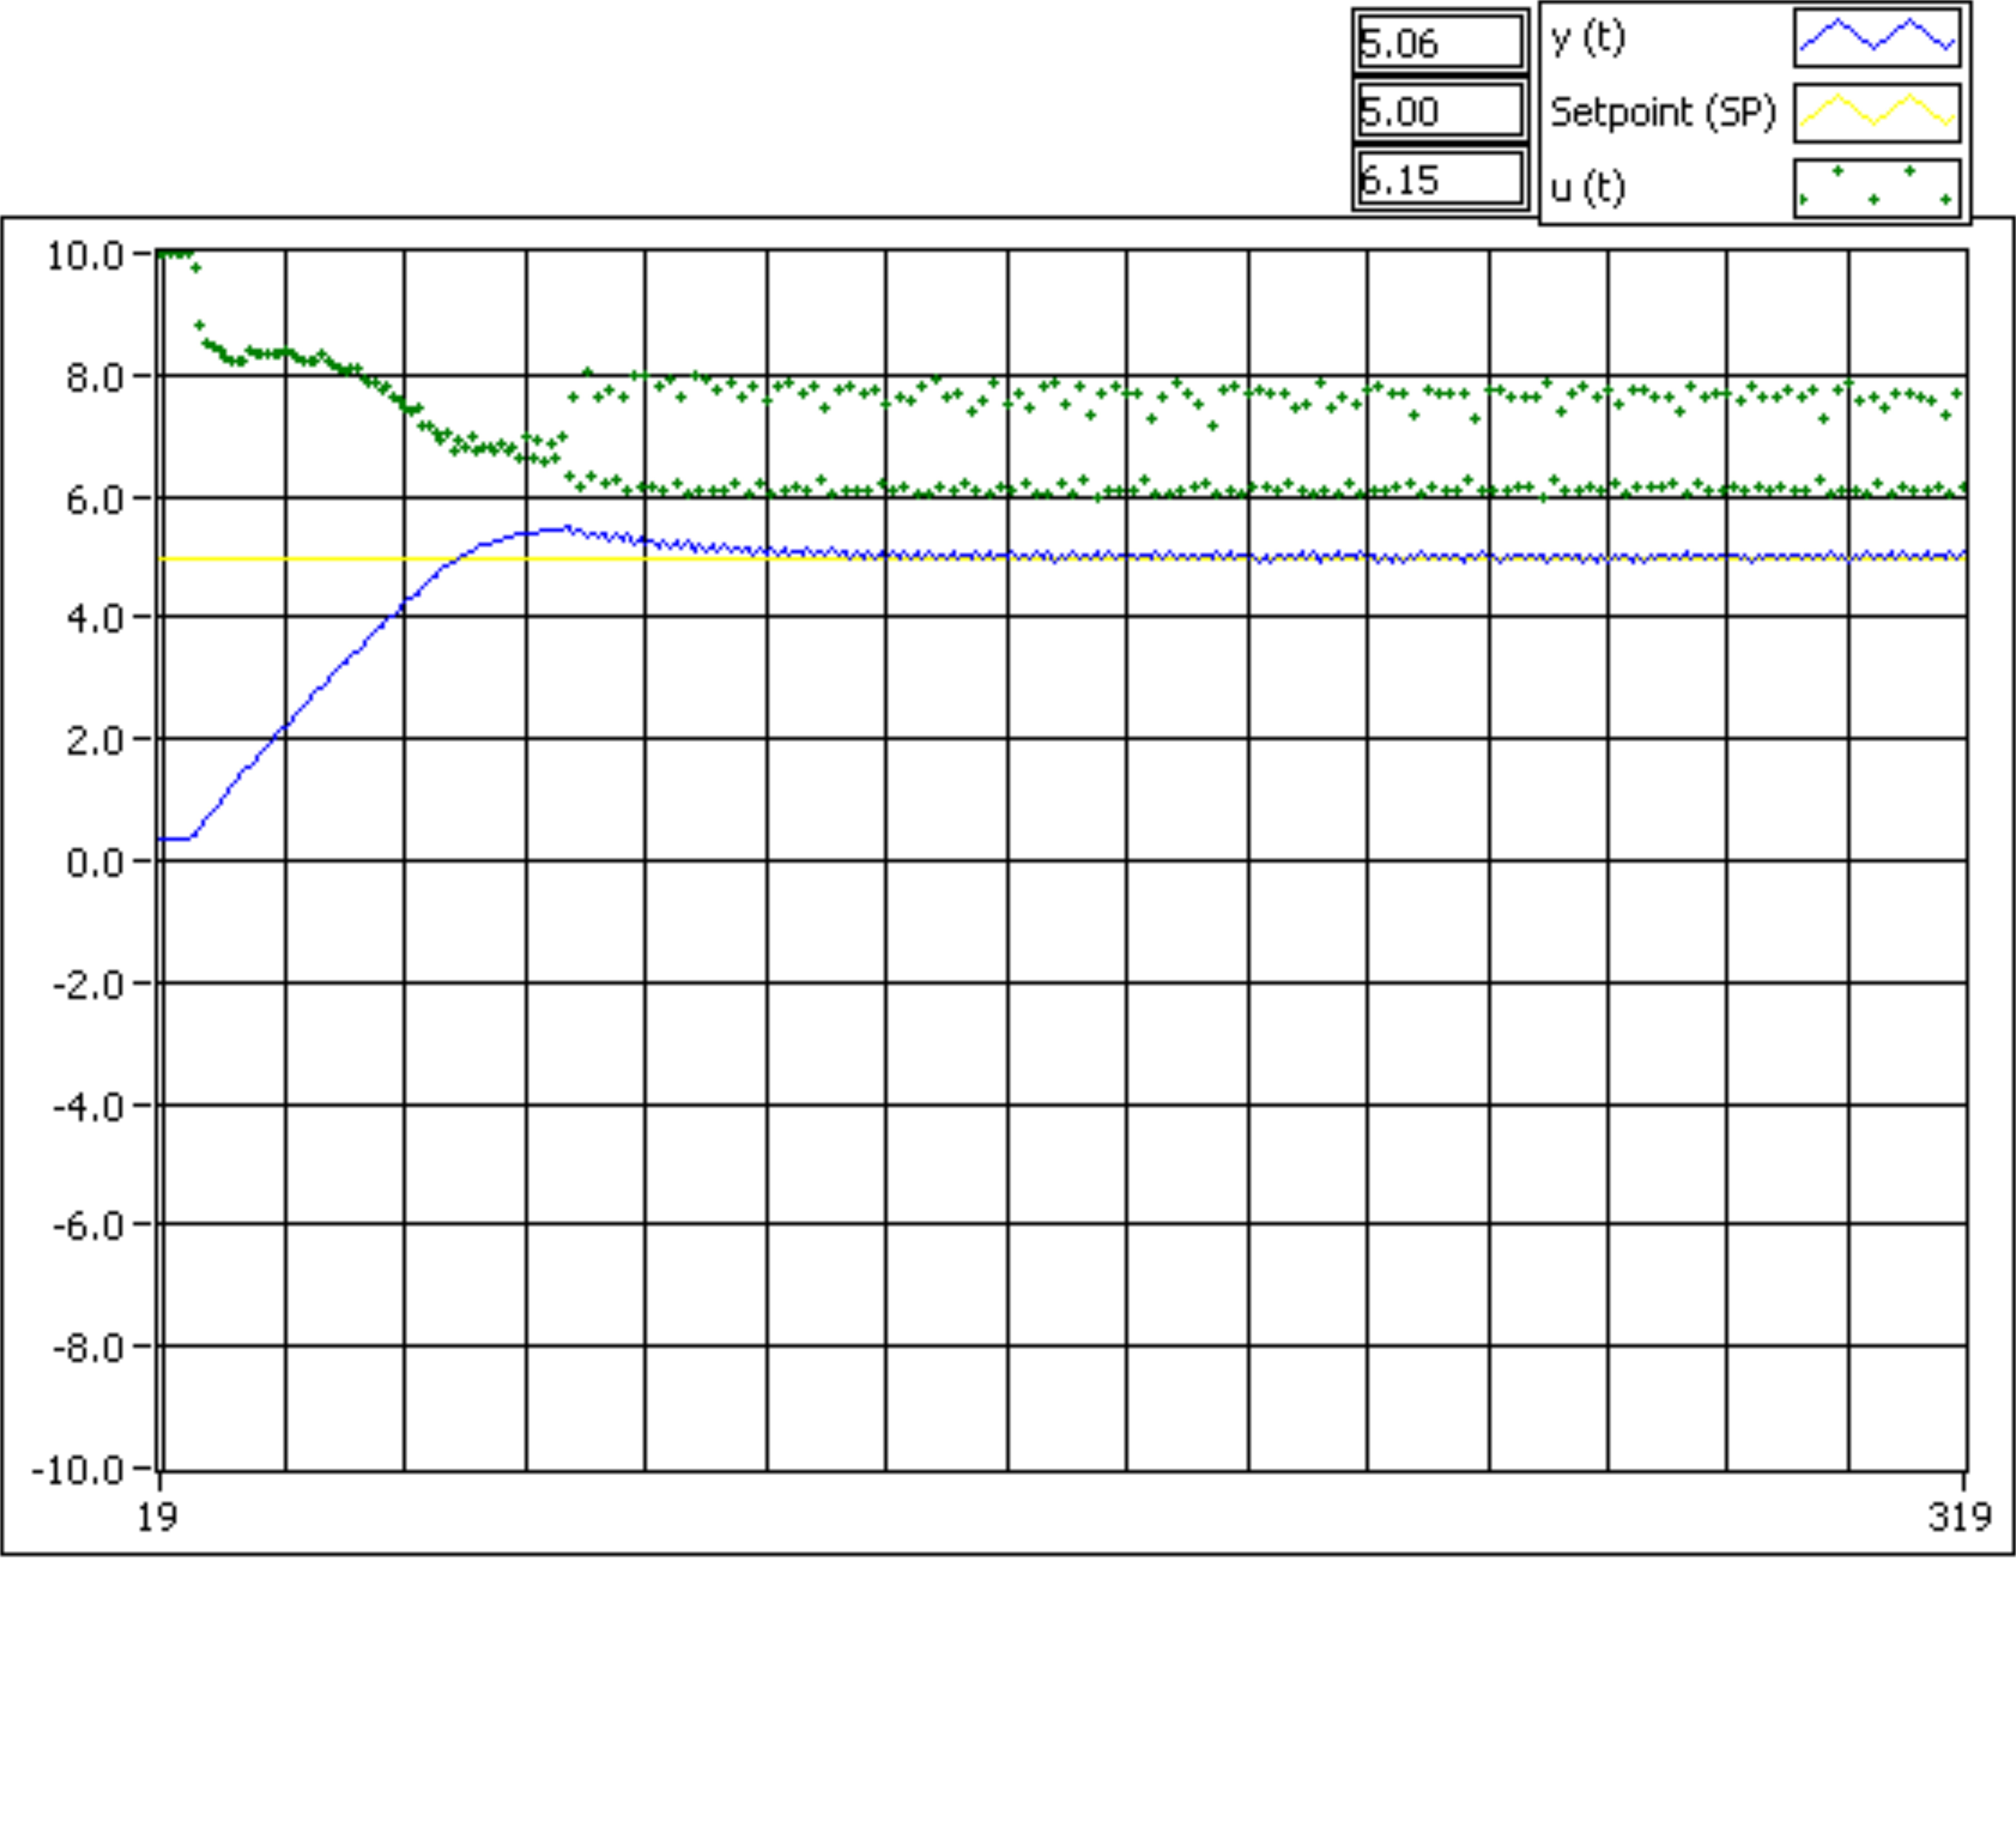
\includegraphics[width=0.6\textwidth]{Imagenes/DigitalE.png}
	\caption{Digital}
	\label{fig:DigitalE}
\end{figure}

















\section{Análisis de Resultados}



\section{Conclusiones}


\section{Referencias}

\bibliographystyle{plain}
\bibliography{Referencias.bib}



\end{document}
